\documentclass{controle}
\usepackage{main}

\title{Baccalauréat général : Épreuve anticipée de mathématiques}
\author{Voie générale : candidats suivant l'enseignement de spécialité de mathématiques}
\date{Durée : 2 heures. L'usage de la calculatrice n'est pas autorisé}

\headrule
\header{Épreuve anticipée de mathématiques}{}{Première Spécialité Mathématiques}
\footer{}{}{Page \thepage{} sur \numpages}
\begin{document}

\begin{coverpages}
\maketitle
\end{coverpages}

\begin{questions}

\titledquestion{Automatismes}[6]

\hfill
\vspace*{0.25cm}

\textbf{Pour cette première partie, aucune justification n'est demandée et une seule réponse est possible par question. Pour chaque question, reportez son numéro dans votre copie et indiquez votre réponse.}

\vspace*{0.25cm}
\begin{parts}
\part L'expression développée réduite de $\left(5x-4\right)^2$ est :\\

\begin{oneparchoices}
\choice $5x^2-16$
\choice $25x^2-16$
\choice $5x^2-40x+16$
\choice $25x^2-40x+16$
\end{oneparchoices}

\vspace{0.8cm}

\part La loi d'interaction gravitationnelle entre deux corps $C_1$ et $C_2$ est : \[F=G\dfrac{m_1m_2}{d^2}\] où $m_1$ et $m_2$ désignent les masses, $d$ la distance entre les deux corps et $G$ la constante gravitationnelle. On a : \\

\begin{oneparchoices}
\choice $d=\dfrac{F-G}{2m_1m_2}$
\choice $d=\sqrt{\dfrac{Gm_1m_2}{F}}$
\choice $d=\dfrac{Gm_1m_2}{F^2}$
\choice $d=\sqrt{\dfrac{F}{Gm_1m_2}}$
\end{oneparchoices}

\vspace{0.8cm}

\part On considère la relation : $A=\dfrac{x+5y}{x}$. Lorsque $x=-\dfrac{2}{3}$ et $y=\dfrac{2}{15}$, la valeur de $A$ est : \\

\begin{oneparchoices}
\choice $\dfrac{2}{3}$ 
\choice $0$
\choice $2$
\choice $-{\dfrac{2}{3}}$
\end{oneparchoices}

\vspace{0.8cm}

\part La fonction $f$ définie sur $\mathbb{R}$ par $f(x)=10x-5$ admet pour tableau de signes :
\begin{center}
\begin{minipage}{0.45\textwidth}
A.\quad
\begin{tabular}{c|ccc}
$x$ & $-\infty$ & $\frac12$ & $+\infty$ \\ \hline
$f(x)$ & $-$ & $0$ & $+$
\end{tabular}
\end{minipage}
\hfill
\begin{minipage}{0.45\textwidth}
B.\quad
\begin{tabular}{c|ccc}
$x$ & $-\infty$ & $\frac12$ & $+\infty$ \\ \hline
$f(x)$ & $+$ & $0$ & $-$
\end{tabular}
\end{minipage}

\vspace{0.8cm}

\begin{minipage}{0.45\textwidth}
C.\quad
\begin{tabular}{c|ccc}
$x$ & $-\infty$ & $2$ & $+\infty$ \\ \hline
$f(x)$ & $-$ & $0$ & $+$
\end{tabular}
\end{minipage}
\hfill
\begin{minipage}{0.45\textwidth}
D.\quad
\begin{tabular}{c|ccc}
$x$ & $-\infty$ & $2$ & $+\infty$ \\ \hline
$f(x)$ & $+$ & $0$ & $-$
\end{tabular}
\end{minipage}

\end{center}

\vspace{0.8cm}

\part On considère $a$, $b$, $c$ des réels non nuls tels que $\dfrac{1}{a}+\dfrac{1}{b}=\dfrac{1}{u}$. On peut affirmer que : \\

\begin{oneparchoices}
\choice $u=a+b$
\choice $u=\dfrac{ab}{a+b}$
\choice $\dfrac{a+b}{ab}$
\choice $u=ab$
\end{oneparchoices}

\vspace{0.8cm}

\part On note $S$ l’ensemble des solutions de l’équation $x^2 = -10$ sur $\mathbb{R}$. On a :

\begin{oneparchoices}
\choice $S=\{-\sqrt{5};\sqrt{5}\}$ 
\choice $S=\{-\sqrt{10};\sqrt{10}\}$
\choice$S=\varnothing$
\choice $S=\{-5;5\}$
\end{oneparchoices}

\vspace{0.8cm}

\part Le prix d'un article augmente de $10\%$ puis il augmente encore de $10\%$. Après ces deux 
évolutions successives, le prix de l'article a augmenté de : 

\begin{oneparchoices}
\choice $\left(10\%\right)^2$
\choice $19\%$
\choice $20\%$
\choice $21\%$
\end{oneparchoices}

\vspace{0.8cm}

\part Si $30\%$ d’une quantité $Y$ vaut $60$, alors la quantité $Y$ vaut :

\begin{oneparchoices}
\choice $Y=1,30 \times 60$
\choice $Y=\dfrac{60}{1,30}$
\choice $Y=\dfrac{60}{0,30}$
\choice $Y=\dfrac{60}{0,70}$
\end{oneparchoices}

\vspace{0.8cm}

\part On a représenté graphiquement ci-dessous une droite dans un repère orthonormé du plan. 

\begin{center}
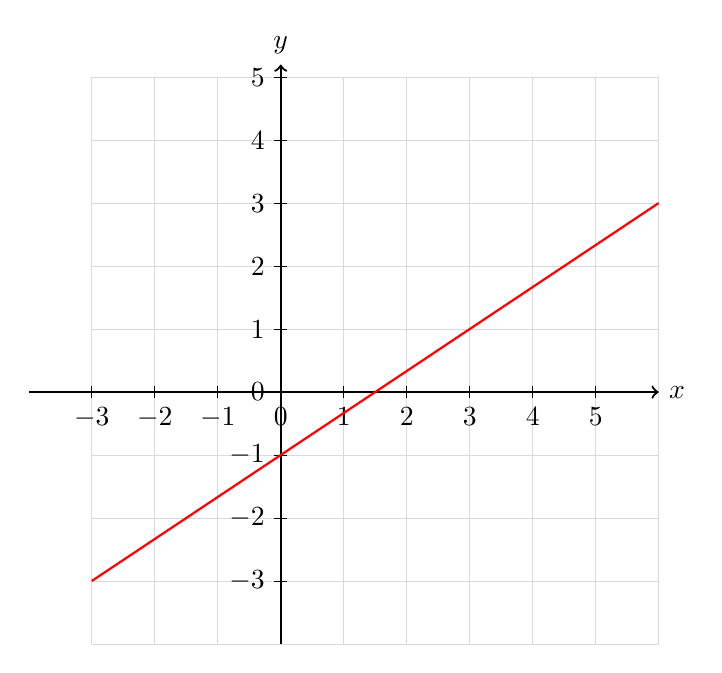
\begin{tikzpicture}[scale=0.8]
  % Grille
  \draw[very thin, color=gray!30] (-3,-4) grid (6,5);

  % Axes
  \draw[->, thick] (-4,0) -- (6,0) node[right] {\(x\)};
  \draw[->, thick] (0,-4) -- (0,5.2) node[above] {\(y\)};

  % Graduations x
  \foreach \x in {-3,-2,...,5}
    \draw (\x,0.1) -- (\x,-0.1) node[below] {\(\x\)};

  % Graduations y
  \foreach \y in {-3,-2,...,5}
    \draw (0.1,\y) -- (-0.1,\y) node[left] {\(\y\)};

  % g(x) = 2 - 1/2x en rouge
  \draw[thick, red, domain=-3:6] plot (\x, {-1 + (2/3)*\x}) node[above left] {};

\end{tikzpicture}
\end{center}

\noindent Une équation de cette droite est :

\begin{oneparchoices}
\choice $y=\dfrac{3}{2}x-1$
\choice $3y-2x+1=0$
\choice $y=-x+\dfrac{2}{3}$
\choice $y-\dfrac{2}{3}x=-1$
\end{oneparchoices}

\vspace{0.8cm}

\part La somme de l'opposé de 2 et de l'inverse de 3 est :

\begin{oneparchoices}
\choice $-\dfrac{5}{3}$
\choice $5$
\choice $6$
\choice $-\dfrac{5}{2}$
\end{oneparchoices}

\vspace{0.8cm}

\part Voici quatre planètes et leur masse.

\begin{center}
\begin{tabular}{|l|c|}
\hline
\textbf{Planète} & \textbf{Masse (en kg)} \\
\hline
Terre   & \num{5973} $\times 10^{21}$ \\
Mercure & \num{33,02} $\times 10^{22}$ \\
Vénus   & \num{48685} $\times 10^{20}$ \\
Mars    & \num{6,4185} $\times 10^{23}$ \\
\hline
\end{tabular}
\end{center}

\noindent La planète dont la masse est la plus importante est :

\begin{oneparchoices}
\choice Terre
\choice Mercure
\choice Vénus
\choice Mars
\end{oneparchoices}

\vspace*{0.8cm}

\part Parmi les listes suivantes, laquelle est susceptible de représenter une suite arithmétique de raison $r=-2$ ?

\begin{choices}
\choice $\left(1;~-2;~4;~-8;~16;~-32;\ldots\right)$ 
\choice $\left(8,2;~6,2;~4,2;~2,2;~0,2;~-1,8; \ldots\right)$ 
\choice $\left(-2;~-4;~-16;~-32;~-64;~-128;~-256; \ldots\right)$ 
\choice $\left(10;~12;~14;~16;~18;~20;\ldots\right)$ 
\end{choices}

\end{parts}

\newpage

\titledquestion{Penser par delà la boite}[7,5]

Messieurs Canu, Langlois et Lavigne construisent une boîte sans convercle pour Madame Abassi, afin qu'elle puisse y jeter ses copies de bac blanc, dont elle fera des boulettes.

Pour ce faire, on part d'une plaque de carton rectangulaire de côtés \qty{24}{\centi\meter} et \qty{15}{\centi\meter}, dont on retire un carré de côté $x$ à chaque coin (voir le patron ci-dessous).
\begin{figure}[!h]
    \centering
    \includegraphics[scale=0.45]{exp1.png}
\end{figure}
\begin{parts}
\part \label{part:Boite} \textbf{Un polynôme de degré 2}

On considère la fonction $P$ définie par l'expression 
\begin{equation*}
P(x)=x^2-13x+30 
\end{equation*}
sur $[0;7,5]$.
\begin{subparts}
\subpart[1] Déterminer les racines de la fonction $P$. 
\subpart[0,5] Dans un repère, dessiner l'allure de la courbe de la fonction $P$, en faisant apparaître ses racines. 
\subpart[0,5] En déduire le tableau de signes de la fonction $P$ sur l'intervalle $[0;7.5]$.
\end{subparts}
\vspace*{0.25cm}

\part \textbf{Expression du volume de la boîte}
%(\textit{Barème : $2=2\times0.25 + 0.5 + 1 $}

On admet que la hauteur de la boîte est $x$, comme le montre le pliage ci-dessous.
\begin{figure}[!h]
\centering
\includegraphics[scale=0.3]{boiterepli.png}
\end{figure}
\begin{subparts}
\subpart[0,5] Exprimer la longueur et la largeur du fond de la boîte en fonction de $x$.%et la hauteur de la boîte en fonction de $x$.
\subpart[0,5] Justifier alors que $x$ prend ses valeurs dans l'intervalle $[0;7,5]$
\subpart[1] Montrer que le volume de la boîte est donné par l'expression
\begin{equation*}
V(x)=4x^3-78x^2+360x\,.
\end{equation*}

\textit{(Rappel : le volume d'un pavé est donné par le produit de sa longueur, de sa largeur et de sa hauteur.)}
\vspace*{0.25cm}
\end{subparts}
\part \textbf{Optimisation du volume} 

\begin{subparts}
\subpart[1] Calculer la dérivée de la fonction $V$, puis vérifier que pour tout $x\in[0;7,5]$, on a
\begin{equation*}
V'(x)=12P(x)\,.
\end{equation*}
\subpart[1] Dresser le tableau de variations de la fonction $V$ sur l'intervalle $[0;7,5]$ (on pourra utiliser les résultats de la partie \ref{part:Boite}).
\subpart[0,5] Quelles sont les dimensions (longueur, largeur, hauteur) de la boîte dont le volume est maximal ? 
\subpart[1] L'ensemble des boulettes de copies de Madame Abassi représente un volume de $500$ $cm^3$ : peut-elle toutes les mettre dans cette boîte ? Justifier.
\end{subparts}
\end{parts}

\vspace*{1cm}

\titledquestion{Suites numériques}[6,5]
Dans le cadre d'une expérience en sociologie, une fausse rumeur sur l'absence d'un professeur est propagée dans le lycée. L'équipe s'installe au début de la journée, et l'expérience commence une heure plus tard, durant laquelle on informe \num{20} personnes. L'équipe observe alors la propagation de la rumeur à chaque heure. Les résultats sont repertoriés dans le graphique suivant :

\vspace*{0.5cm}
\begin{center}
\tikzset{every mark/.append style={scale=2,thick,color=black}}
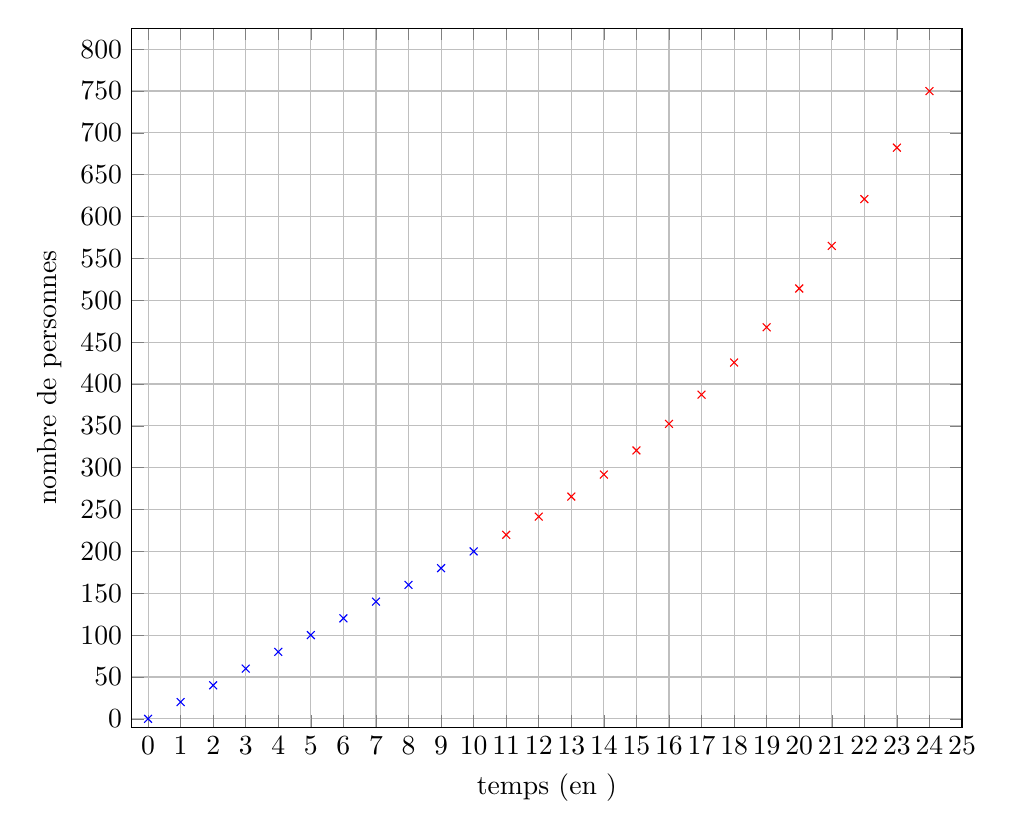
\begin{tikzpicture}
\begin{axis}[
  xmin=-0.5,
  xmax=25,
  ymin=-10,
  ymax=825,
  xlabel= temps (en \unit{\hour}),
  ylabel=nombre de personnes,
  width=\textwidth,
  grid=both,
  xtick distance=1,
  ytick distance=50
]
\addplot+[samples=11, domain=0:10, only marks, mark=x] {20*x};
\addplot+[samples=14, domain=11:24, only marks, mark=x] {200*(1.099)^(x-10)};
\end{axis}
\end{tikzpicture}
\end{center}
\begin{parts}
\part
\begin{subparts}
\subpart[0.5] Combien de personnes sont informées \qty{5}{\hour} après le début de la propagation de la rumeur ?
\subpart[0.5] L'intégralité des personnes au sein de ce lycée est informée de la rumeur au bout de \qty{24}{\hour}. Combien y a-t-il de personnes au sein de ce lycée ?
\subpart[0.5] À partir de combien de temps le nombre de personnes informées devient supérieur à \num{450} ?
\end{subparts}
\part Une suite arithmétique semble modéliser l'évolution de la propagation de la rumeur durant les dix premières heures. On note $a_n$ le nombre de personnes informées après $n$ heures.
\begin{subparts}
\subpart[0.5] Donner les termes $a_0$ et $a_1$ à partir des données de l'énoncé et du graphique.  
\subpart[0.5] On admet que sa raison est de $20$. En déduire l'expression de $a_n$ en fonction de $n$.
\subpart[0.5] En déduire que $a_{10} = 200$.
\end{subparts}
\part On souhaite modéliser la suite de la propagation à partir de \qty{10}{\hour}. On constate qu'à partir de \qty{10}{\hour}, le nombre de personnes informées augmente d'environ \num{9,9}\% chaque heure supplémentaire. On note $g_n$ le nombre de personnes informées à $10 + n$ heures.
\begin{subparts}
\subpart[0.5] Justifier que $g_0 = a_{10} = 200$.
\subpart[0.5] Justifier que pour tout $n \in \N$, $g_{n+1} = 1,099 \times g_n$. Quelle est la nature de $(g_n)_{n \in \N}$ ?
\subpart[0.5] En déduire une expression de $g_n$ en fonction de $n$.
\subpart[1] Pour quel indice $n$ le terme $g_n$ correspond au nombre de personnes informées au bout de \qty{24}{\hour}, c'est-à-dire \textbf{depuis le début de la propagation de la rumeur} ? Le calculer à l'aide du tableau des puissances de \num{1,099}.
\subpart[1] En admettant que l'expérience continue au-delà de \qty{24}{\hour} dans un lycée présentant un nombre plus élevé de personnes, à partir de combien d'heures le nombre de personnes informées est supérieur à \num{1000}.

\begin{table}[htbp]
\centering
\begin{tabular}{|c|*{11}{c|}}
\hline
$n$ & 0 & 1 & 2 & 3 & 4 & 5 & 6 & 7 & 8 & 9\\ \hline
$1,099^n$ & 1.000 & 1.099 & 1.207 & 1.327 & 1.459 & 1.603 & 1.762 & 1.936 & 2.128 & 2.239\\ \hline 
\end{tabular}
\vspace*{0.5cm}

\begin{tabular}{|*{11}{c|}}
\hline
10 & 11 & 12 & 13 & 14 & 15 & 16 & 17 & 18 & 19 & 20 \\ \hline
2.570 & 2.825 & 3.104 & 3.412 & 4.749 & 4.121 & 4.529 & 4.977 & 5.470 & 6.011 & 6.606 \\ \hline
\end{tabular}
\caption*{\textit{Tableau de puissances de \num{1.099}}}
\end{table}



\end{subparts}
\end{parts}
\end{questions}
\end{document}